\documentclass[10pt,a4paper]{report}
\usepackage[utf8]{inputenc}
\usepackage[russian]{babel}
\usepackage[OT1]{fontenc}
\usepackage{amsmath}
\usepackage{amsfonts}
\usepackage{amssymb}
\usepackage{graphicx}
\author{Киселев Антон и Кенть Никита}
\title{Отчет по лабораторной работе по дисциплине: "Сети и системы передачи данных"\newline
тема: "Визуализация сигналов во временной и частотной области"}
\date{13.03.14}
\begin{document}
\maketitle
\pagebreak
\chapter{Теоретическая часть}
\section{Цель работы}
Познакомиться со средствами генерации сигналов и визуализации их спектров.
\section{Постановка задачи}
В командном окне MATLAB и в среде Simulink промоделировать чистый синусоидальный сигнал, 
так же синусоидальный сигнал с шумом. Получить их спектры.

\chapter{Ход работы}
\section{Алгоритм работы}
\begin{itemize}
\item Построение синусоидального сигнала без шумов
\item Вывод временной характеристики сигнала
\item Реализация  преобразования Фурье 
\item Построение графика спектральной плотности 
\item Построение зашумленного синусоидального сигнала  
\item Вывод временной характеристики полученного сигнала
\item Преобразования Фурье 
\item Построение графика спектральной плотности для зашумленного сигнала
\end{itemize}
\section{Код MATLAB}
function main()\newline
x=0:0.01:4*pi;\newline
t0 = 5;\newline
\%исходный сигнал\newline
y = sin(2*pi*f0*x);\newline
figure(1)\newline
plot(x(1:200),y(1:200))\newline
grid\newline
\%спектр исходного сигнала\newline
figure(2)\newline
spectrum = fft(y,1024);\newline
normspectrum = spectrum.*conj(spectrum)/1024;\newline
f=100*(0:1023)/1024;\newline
plot(f, normspectrum(1:1024))\newline
axis([0 max(f) 0 10])\newline
grid\newline
\%зашумленный сигнал\newline
ynoize = y+ 0.5*rand(size(x));\newline
figure(3)\newline
plot(x(1:200),ynoize(1:200));\newline
grid\newline
\%спектр зашумленного сигнала\newline
spectrum = fft(ynoize,1024);\newline
noizespectrum = spectrum.*conj(spectrum)/1024;\newline
figure(4)\newline
plot(f, noizespectrum())\newline
axis([0 max(f) 0 10])\newline
grid\newline
\section{Результаты работы}
В результате выполнения программы получились графики временной и частотной характеристик исходного и зашумленного синусоидальных сигналов. \newpage
\begin{figure}
\begin{center}
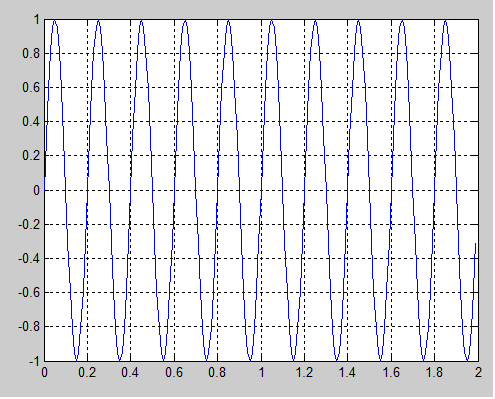
\includegraphics[angle=0, scale = 0.9]{1.png}\newline
рис. 1 Исходный сигнал\newline
\end{center}
\begin{center}
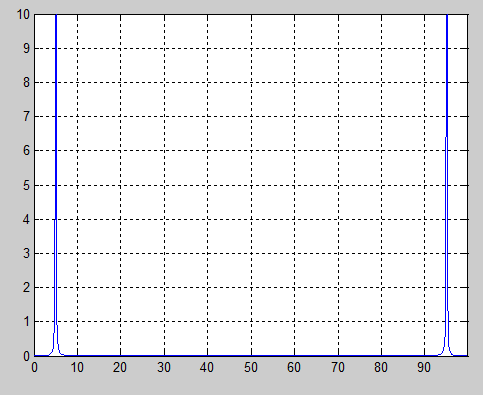
\includegraphics[angle=0, scale = 0.9]{2.png}\newline
рис. 2. Спектр исходного сигнала\newline
\end{center}
\end{figure}
\begin{figure}
\begin{center}
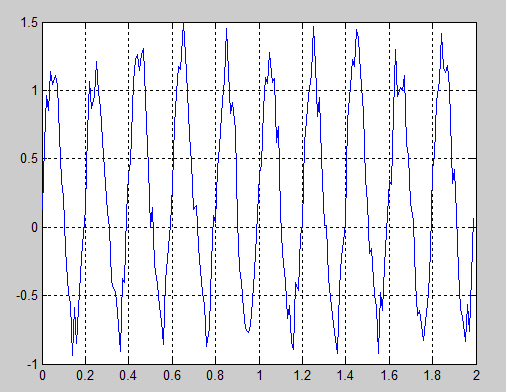
\includegraphics[angle=0, scale = 0.9]{3.png}\newline
рис. 3. Зашумленный сигнал\newline
\end{center}
\begin{center}
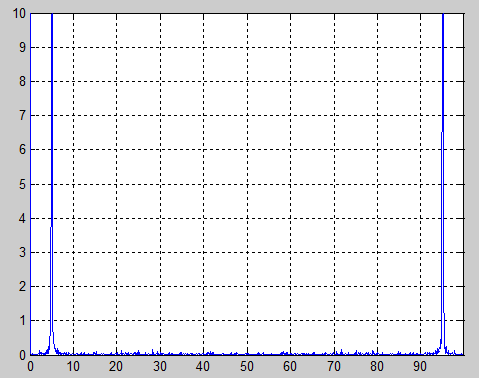
\includegraphics[angle=0, scale = 0.9]{4.png}\newline
рис. 4. Спектр зашумленного сигнала\newline
\end{center}
\end{figure}
\chapter{Вывод}
В данной лабораторной работе был получен спектр исходного сигнала синуса. Спектр представляет собой два резко возрастающих на коротком промежутке графика, симметрично расположенных на оси. Исходный сигнал был зашумлен, его график представляет собой "неровный" синус. Также был получен спектр зашумленного сигнала, который представляет собой "неровный" спектр исходного сигнала.
\end{document}
